\documentclass[12pt]{article}
\usepackage{amsmath}
\usepackage{graphicx,psfrag,epsf}
\usepackage{enumerate}
\usepackage{natbib}
\usepackage[spanish]{babel}
\selectlanguage{spanish}
\usepackage[utf8]{inputenc}
\usepackage{xcolor}
\usepackage{textcomp}
\usepackage{hyperref}
\usepackage[ruled,linesnumbered]{algorithm2e}

\newcommand{\blind}{0}

\usepackage{mathtools}
\usepackage{listings}             % Include the listings-package
\lstset{ % General setup for the package
	language=Perl,
	basicstyle=\small\sffamily,
	numbers=left,
 	numberstyle=\tiny,
	frame=tb,
	tabsize=4,
	columns=fixed,
	showstringspaces=false,
	showtabs=false,
	keepspaces,
	commentstyle=\color{red},
	keywordstyle=\color{blue}
}

\addtolength{\oddsidemargin}{-.75in}%
\addtolength{\evensidemargin}{-.75in}%
\addtolength{\textwidth}{1.5in}%
\addtolength{\textheight}{1.3in}%
\addtolength{\topmargin}{-.8in}%


\begin{document}


%\bibliographystyle{natbib}

\def\spacingset#1{\renewcommand{\baselinestretch}%
{#1}\small\normalsize} \spacingset{1}


%%%%%%%%%%%%%%%%%%%%%%%%%%%%%%%%%%%%%%%%%%%%%%%%%%%%%%%%%%%%%%%%%%%%%%%%%%%%%%

\if0\blind
{
  \title{\bf Paralelización de la Factorización $QR$ por Tiles}
  \author{Mihaita Alexandru Lupoiu\hspace{.2cm}\\
    Computación Paralela y Distribuida, Universidad Politécnica de Valencia}
  \maketitle
} \fi

\if1\blind
{
  \bigskip
  \bigskip
  \bigskip
  \begin{center}
    {\LARGE\bf Factorización $QR$ por Tiles}
\end{center}
  \medskip
} \fi

\bigskip
\begin{abstract}

Los sistemas multinúcleo están continuamente ganando terreno en el mundo de la informática generál y más aún cuando se trata de High Performance Computing. Por esa razón los algoritmos de álgebra lineal deben ser reformulados o se deben desarrollar nuevos algoritmos con el fin de tomar ventaja de las características arquitectónicas de estos nuevos procesadores. Este trabajo está basado en las Working Notes 190[2] y 191[3] de LAPACK que presenta un algoritmo para la factorización QR, donde las operaciones se pueden representar como una secuencia de tareas pequeñas que operan por bloques.



%Paralelismo de grano fino se convierte en un requisito importante e introduce la necesidad de la sincronización suelto en la ejecución paralela de una operación. 
 

Estas tareas se pueden organizar de forma dinámica y la ejecución se realiza en base a las dependencias entre ellas y en la disponibilidad de recursos computacionales. Esto puede dar lugar a una ejecución fuera de orden de las tareas que ocultarán completamente la presencia de tareas secuenciales intrinsicas en la factorización.

% Comparaciones de rendimiento se presentan con el algoritmo LAPACK para factorización QR, donde el paralelismo sólo se puede aprovechar en el plano de las operaciones BLAS.


%El creciente número de núcleos en las arquitecturas modernas y el incremento de los nodos de los centros de datos, requiere el desarrollo de nuevos algoritmos como un medio para la consecución de concurrencia y por lo tanto la escalabilidad. Este trabajo presenta un algoritmo para calcular la factorización $LDL^T$ de matrices simétricas indefinidas sin utilizar pivotamiento. 
  
  \end{abstract}

\noindent%
{\it Keywords:}  $QR$, matriz, factorización, LAPACK, paralelización, BLAS.

\spacingset{1.45}
\section{Introduction}
\label{sec:intro}

En este trabajo se analizarán las tecnicas y propuestas de algoritmos para realizar la factorización QR por ''tiles''. Más en concreto se centrá en los articulos ''Working Notes 190'' y ''Working Notes 191'' de LAPACK.

El trabajo explicará en que consiste la Factorización QR por Bloques para posteriormente explicar en la segunda parte como se ha planteado la realización de la Factorización QR por Tiles. Para acabar se explicará la implementación que se ha intentado realizar del mismo.

\section{La Factorización $QR$ por Bloques}
\label{sec:block_qr}

La factorización QR es una transformación que factoriza una matríz inicial $A$ de tamaño $m \times n$ en dos matrices $Q$ y $R$ donde $Q$ es una matríz unitaria de tamaño $n \times n$ y $R$ es una matriz triangular de tamaño $m \times m$. 

Esta factorizacion se realiza aplicando $min(m,n)$ reflexiones de Householder a la matriz $A$. Como las refleciones de Householder son transformaciones ortogonales, esta factorización es más estable comparado con la LU pero a cambio de una mayor coste computacional. La factorización QR tiene un coste de $2n^2(m-n/3)$ Flops, mientras que la LU tiene un coste de $n^2(m-n/3)$ FLops.

En la librería de LAPACK se utiliza una versión peculiar de la factorización QR que consigue mejores prestaciones en arquitecturas con varios niveles de memória gracias a la división por bloques. 

Este algoritmo se basa en acumular una cantidad de transformaciónes de 
Householder y se denominado {\it panel factorization}, que luego se aplica todas a la vez aprovechando las rutinas de BLAS de nivel 3. Esta técnica utilizada para acumular las transformaciones de householder se denomina técnica compacta WY.

La rutina de LAPACK que realiza la factorización QR se denomina \texttt{DGEQRF} y se explicará a continuación.%http://www.netlib.no/netlib/lapack/double/dgeqrf.f

Consideranto una matriz $A$ de tamaño $m \times n$ que se puede reprezentar como:
\begin{displaymath}
  A=\left(\begin{array}{cc}
    A_{11} & A_{12}  \\
    A_{21} & A_{22}  \\
  \end{array}\right)
\end{displaymath}
Donde:
\begin{itemize}
  \item $A_{11}$ es de tamaño $b \times b$
  \item $A_{12}$ es de tamaño $b \times (n-b)$
  \item $A_{21}$ es de tamaño $(m-b) \times b$
  \item $A_{22}$ es de tamaño $(m-b) \times (n-b)$
\end{itemize}

El algoritmo de LAPACK para realizar al factorización QR se puede describir como una secuencia de pasos, y cada paso consiste en realizar la transformación de la Ecuación (1):

\begin{equation}
  \label{eq:lap_qr0}
  A=\left(\begin{array}{cc}
    A_{11} & A_{12}  \\
    A_{21} & A_{22}  \\
  \end{array}\right) \Longrightarrow
  \left(\begin{array}{c}
      V_{11} \\
      V_{21}
\end{array}\right), \left(\begin{array}{cc}

    R_{11}   & R_{12}        \\
      0     &\tilde{A}_{22} \\
  \end{array}\right)
\end{equation}

La transfromación de la Equación (1) se obtiene en dos pasos:

\begin{enumerate}
\item {\bf Factorización del Panel.} En este paso se realiza una transformación QR del panel $(A_{*1})$ como se puede observar en la Equation~\eqref{eq:lap_qr1}.
  \begin{equation}
    \label{eq:lap_qr1}
    \left(\begin{array}{c}
        A_{11} \\
        A_{21}
      \end{array}\right) \Longrightarrow
    \left(\begin{array}{c}
        V_{11} \\
        V_{21}
      \end{array}\right), (T_{11}), (R_{11})
  \end{equation}
  Esta operación produce $b$ reflexiones de Householder $(V_{*,1})$ y 
una matriz triangular superior $R_{11}$ de tamaño $b \times b$ que representa una parte de la matriz final $R$, mediante la rutina \texttt{DGEQR2} disponible en LAPACK. También en este paso se genera la matriz triangular $T_{11}$ de tamaño $b \times b$ mediante la rutina \texttt{DLARFT} también disponible en LAPACK. La matriz $V_{11}$ es una matriz triangular inforior unitaria de tamaño $b \times b$. Los arrays de $V_{*1}$ y $R_{11}$ no tenecesitan espacio extra dado que sobre-escriben $A_{*1}$, pero se encesita un espacio temporal de trabajo para $T_{11}$.

\item {\bf Actualizacion de la submatriz.} En este paso la transformación realizada en el apartado anterior es aplicado al resto de matriz como se puede observar en la Equacion~\eqref{eq:lap_qr2}.
  \begin{equation}
    \label{eq:lap_qr2}
    \left(\begin{array}{c}
        R_{12}       \\
        \tilde{A}_{22}\\
      \end{array}\right) =
    \left(\begin{array}{c}
        \\
        \\
      \end{array}\right.  I - \left(\begin{array}{c}
        V_{11} \\
        V_{21}
      \end{array}\right) \begin{array}{c}
      \cdot (T_{11}) \cdot\\
      \\
    \end{array}   \begin{array}{cc}
      (V^T_{11}& V^T_{21}) \\
      &          \\
    \end{array}\left.\begin{array}{c}
        \\
        \\
      \end{array}\right)  \left(\begin{array}{c}
        A_{12}  \\
        A_{22}  \\
      \end{array}\right)
  \end{equation}
    Esta operacion se realiza mediante la rutina de LAPACK \texttt{DLARFB} y genera la matriz $R_{12}$ de tamaño $b \times (n-b)$, que es una parte de la matriz final de $R$ y una matriz $\tilde{A}_{22}$.
\end{enumerate}

Esta transfromación~\eqref{eq:lap_qr0} se vuelve a repetir pero esta vez a la submatriz $\tilde{A}_{22}$ y así succesivamente hasta que se llega al final de la matriz $A$.

EL valor de $b \ll m,n$ por defecto tiene el valor de 32 en LAPACK-3.1.1, pero este valor se puede modificar para intentar buscar uno más optimo dependiendo de las caracteristicas de la arquitectura.

%%%%%%%%%%%%%%%%%

\section{Tiled QR Factorization}
\label{sec:tiled}

La idea de distribución dinamica y la ejecución fuera de orden de las tareas se puede aplicar a toda clase de algoritmos que permiten la paralelización de las operaciones de Álgebra Lineal comunes. Un ejemplo es la factorización de Cholesky, que no es necesario realizar ningún cambio algorítmico ya que se puede paralelizar de forma natural por''tiles''. Mientras que el algoritmo por bloque de la factorizacion QR tiene un cuello de botella computacional por el tipo de matriz que se emplean. Con el fin de tener una mayor granularidad en la QR, las operaciones se tienen que paralelizar por tareas y por lo tanto se va a necesitar un cambio algorítmico importante en la QR. 

El cambio algorítmico que se propone en el artículo ''Working Notes 191''es el siguiente:


%%%%%%%%%%%%%%%

Suponeindo que la matriz $A$ es de tamaño $pb \times qb$
\begin{displaymath}
  \left(\begin{array}[!h]{cccc}
    A_{11}  & A_{12} & \dots  & A_{1q}  \\
    A_{21}  & A_{22} & \dots  & A_{2q}  \\
    \vdots &       & \ddots & \vdots \\
    A_{p1}  & A_{p2} & \dots  & A_{pq}
  \end{array}\right)
\end{displaymath}
donde $b$ es el tamaño de bloque para cada $A_{ij}$ de tamaño $b \times b$, la factorización QR se puede realizar mediante el Algoritmo~\ref{alg1}.

\begin{algorithm}[H]
   \SetAlgoLined
         \For{$k=1, 2..., min(p,q)$}{
   	        %\texttt{DGEQT2}($A_{kk}$, $T_{kk}$);\\
   	        \texttt{DGEQRT}($A_{kk}$, $V_{kk}$, $R_{kk}$, $T_{kk}$);\\
   	        \For{$j=k+1, k+2, ..., q$}{
       	        %\texttt{DLARFB}($A_{kj}$, $V_{kk}$, $T_{kk}$);\\
       	        \texttt{DLARFB}($A_{kj}$, $V_{kk}$, $T_{kk}$, $R_{kj}$);
   	        }
   	        \For{$i=k+1, k+1, ..., p$}{
       	        %\texttt{DTSQT2}($R_{kk}$, $A_{ik}$, $T_{ik}$);\\
       	        \texttt{DTSQRT}($R_{kk}$, $A_{ik}$, $V_{ik}$, $T_{ik}$);\\
       	        \For{$i=k+1, k+1, ..., p$}{
       	            %\texttt{DSSRFB}($A_{kj}$, $A_{ij}$, $V_{ik}$, $T_{ik}$);\\
       	            \texttt{DSSRFB}($R_{kj}$, $A_{ij}$, $V_{ik}$, $T_{ik}$);
   	            }
   	        }
   	    }
   		
   \label{alg1}
   \caption{\textsc{Algoritmo de la factorización QR por Bloques.}}
\end{algorithm}


Como se puede observar en la Figura.~\ref{alg1}, la factorización QR por bloques se basa en las siguientes cuatro operaciones:

\begin{description}
\item[\texttt{DGEQRT}.] Esta subrutina se utiliza para realizar la factorización QR por bloques del bloque $A_{kk}$ de tamaño $b \times b$. El tamaño de bloque interno es $s$. El resultado de esta operacion es una matriz triangular superior $R_{kk}$, una matriz triangular infoerior $V_{kk}$ que contiene las $b$ reflexiones de Householder y una matriz triangular superior $T_{kk}$  como fue definida por la tecnica de WY para acumular las transformaciones. Esta subrutina se basa en la DGEQRF de LAPACK, por lo que aprovecha las rutinas de BLAS 3.

  \texttt{DGEQRT}($A_{kk}$, $V_{kk}$, $R_{kk}$, $T_{kk}$):
  \begin{displaymath}
    A_{kk} \longrightarrow (V_{kk}, R_{kk}, T_{kk})=QR(A_{kk})
  \end{displaymath}

\item[\texttt{DLARFB}.] Esta subrutina de LAPACK basado en BLAS 3 se utiliza para aplicar las transformacion de $(V_{kk}, T_{kk})$ realizadas por la subritina \texttt{DGEQRT} al bloque $A_{kj}$ generando $R_{kj}$.

  \texttt{DLARFB}($A_{kj}$, $V_{kk}$, $T_{kk}$, $R_{kj}$):
  \begin{displaymath}
    A_{kj}, V_{kk}, T_{kk} \longrightarrow R_{kj}=(I-V_{kk}T_{kk}V^T_{kk})A_{kj}
  \end{displaymath}

\item[\texttt{DTSQRT}.] Esta subrutina realiza la factorización QR por bloques que se aplica al bloque $R_{kk}$ (submatriz triangular superior) y al bloque $A_{ik}$ de forma conjunta. Esta subrutina devolverá una matriz triangular superior $\tilde{R}_{kk}$ que contiene las $b$ reflexiones de Householder, donde $b$ es el tamaño del bloque. También se crea una matriz triangular superior $T_{ik}$ definida por la tecnica de WY comprimido para cumular las transformaciones de householder.
 
  \texttt{DTSQRT}($R_{kk}$, $A_{ik}$, $V_{ik}$, $T_{ik}$):
  \begin{displaymath}
    \left(
      \begin{array}[!h]{c}
        R_{kk}\\
        A_{ik}
      \end{array}\right) \longrightarrow
        (V_{ik}, T_{ik}, R_{kk})=QR\left(\begin{array}[!h]{c}
        R_{kk}\\
        A_{ik}
      \end{array}\right)
  \end{displaymath}


\item[\texttt{DSSRFB}.] Esta subrutina actualiza la matriz formada por los dos bloques $A_{kj}$ y $A_{ij}$, después de aplicar transformaciones realizadas por \texttt{DTSQRT} 
  
  \texttt{DSSRFB}($R_{kj}$, $A_{ij}$, $V_{ik}$, $T_{ik}$):
  \begin{displaymath}
    \left(\begin{array}{c}
      R_{kj}\\
      A_{ij}
    \end{array}\right), V_{ik}, T_{ik} \longrightarrow
    \left(
    \begin{array}{c}
      R_{kj}\\
      A_{ij}\\
    \end{array}\right)=
    (I - V_{ik}T_{ik} V^T_{ik})\left(\begin{array}{c}
      R_{kj}\\
      A_{ij}
    \end{array}\right)
  \end{displaymath}
  
\end{description}


\clearpage

\begin{figure}[!h]
  \begin{center}
    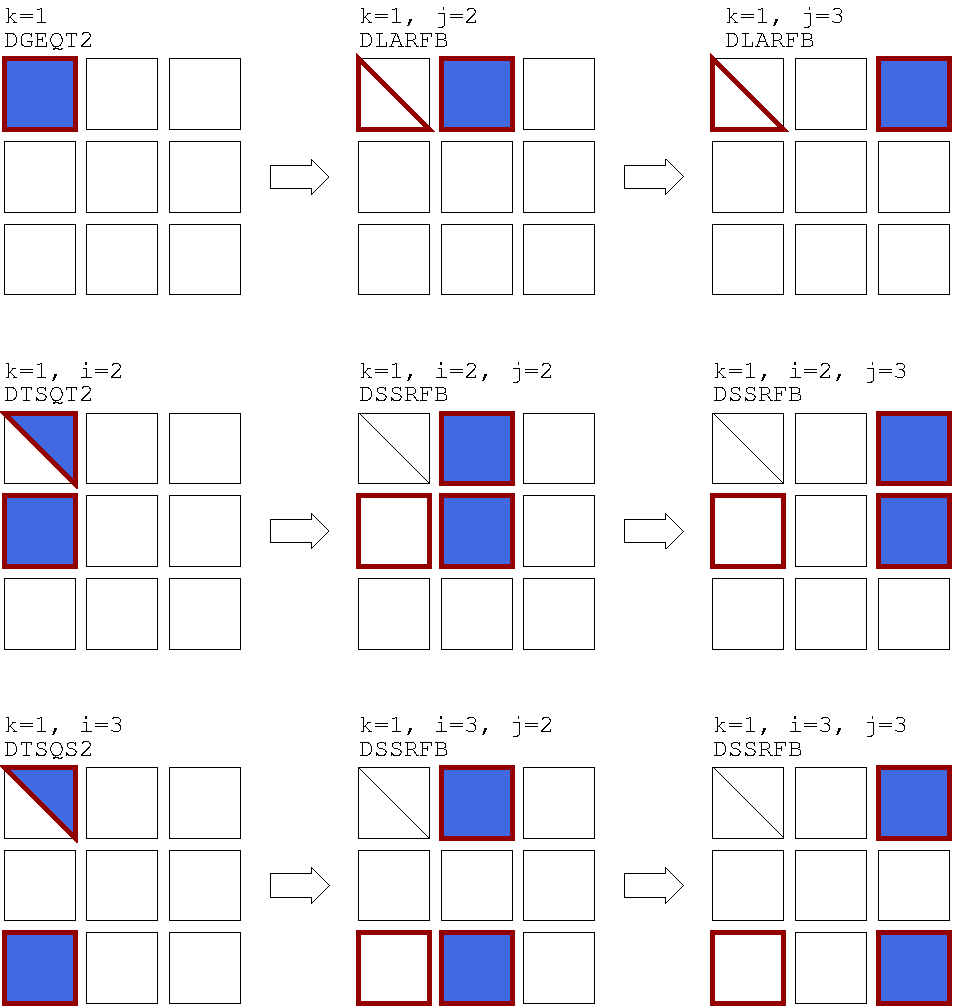
\includegraphics[width=\textwidth]{images/blk_alg_col.pdf}
  \caption{\label{fig:blk_alg}Graphical representation of one     repetition of the outer loop in Algorithm~\ref{alg1} on a matrix with $p=q=3$.
}
  \end{center}
\end{figure}

\clearpage

La figura~\ref{fig:blk_alg} Es una representación grafica de una de las repeticiones ($k=1$) del algoritmo~\ref{alg1}, donde $p=q=3$. Los bordes rojos representan que bloques de la matriz se están leyendo y la area azul de los bloques representa los lugares donde se está escribiendo en la matriz. Las matrices $T_{kk}$ no se muestran en esta figura para evitar confusiones. 

El algoritmo~\ref{alg1} se puede representar como un Grafo Acíclico dirigido (DAG) donde los nodos representar tareas que se aplican en los bloques de tamaño $b \times b$ y las aristas representan las dependencias. 

\begin{figure}[!h]
  \begin{center}
    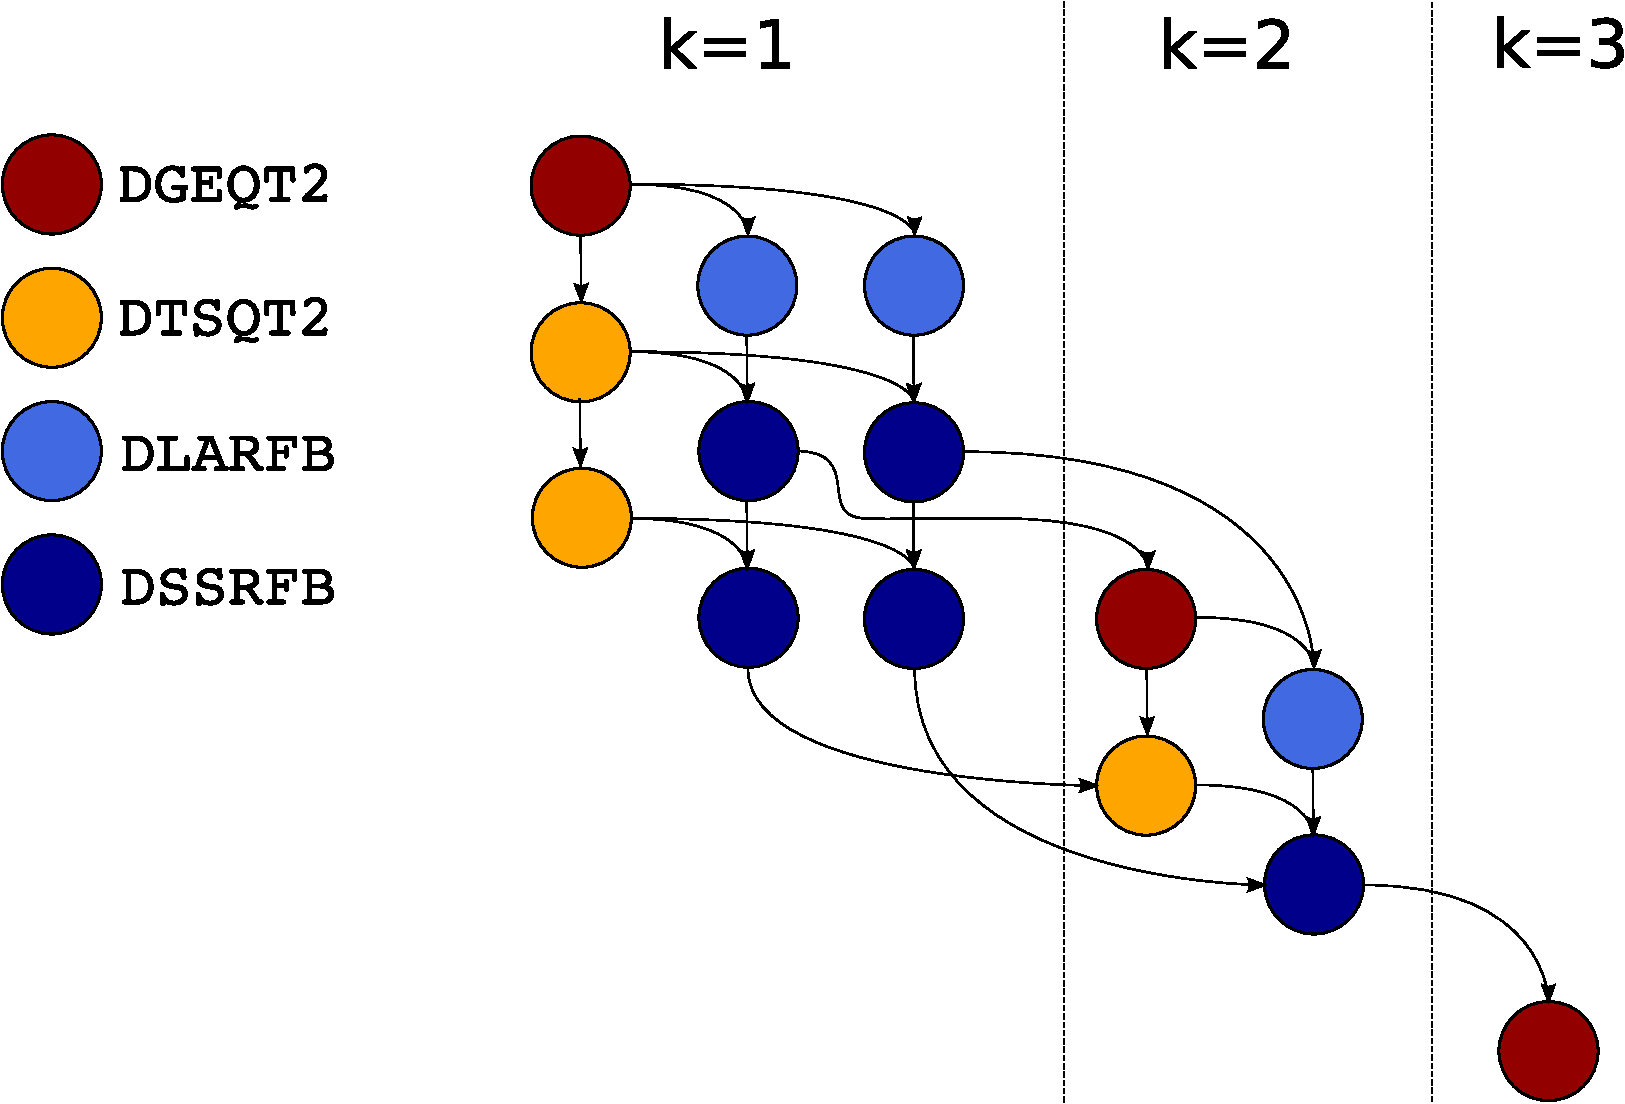
\includegraphics[width=\textwidth]{images/qr_dag_3x3_color.pdf}
  \caption{\label{fig:qr_dag}The dependency graph of
    Algorithm~\ref{alg:blkqr} on a matrix with $p=q=3$.}
  \end{center}
\end{figure}


La figura~\ref{fig:qr_dag} muestra el DAG del algoritmo~\ref{alg1}, que una vez conocido, las tareas se pueden distribuir de forma asincrona mientras las dependencias entre ellas no son violadas. Una parte clitica es identificar en el DAG es encontrar que nodos tienen mayor numero de aristas, dado que en base a esa observación se le puede asignar mayor prioridad a los nodos que calculan bloques criticos. En este caso los bloques que están calculando la factorización QR con la rutina \texttt{DGEQRT} tiene la prioridad más alta y el resto de tareas \texttt{DLARFB}, \texttt{DTSQRT}, \texttt{DSSRFB} se le puede asignar una prioridad descendente.


\clearpage

\section{Implementación}
\label{sec:impl}

A la hora de realizar la implementación fue el hecho de encontrar las rutinas del LAPACK para poder utilizarlas. El nombre de estas rutinas se habían cambiado y tras hablar con Alfredo Buttari\footnote{Uno de los autores de los articulos}, descubrí que las rutinas que tengo que utilizar son las siguientes:

\begin{itemize}
  \item DGEQRT
  \item DGEMQRT que coresponde a DLARFB
  \item DTPQRT que coresponde a DTSQRT
  \item DTPMQRT que coresponde a DSSRFB
\end{itemize}

Tambíen cabe destacar que estas funciones requieren que la librería de LAPACK este en una versión más recientes(3.5.0). Para la instalación se puede utilizar el siguiente script:

Código:
\begin{lstlisting}[basicstyle=\ttfamily\tiny]
%\begin{lstlisting}[basicstyle=\ttfamily]
#!/bin/bash

sudo apt-get update
sudo apt-get install make
sudo apt-get install gcc
sudo apt-get install liblapack-dev
sudo apt-get install liblapack3
sudo apt-get install libopenblas-base
sudo apt-get install libopenblas-dev
\end{lstlisting}

Una vez instalado y comprobado que funciona el algoritmo, se tuvo que preparar la matriz de entrada para que se pueda procesar por bloques. El codigo corespondiente sería el siguiente:

\begin{lstlisting}[basicstyle=\ttfamily\tiny]
void convtile(double *A, double *B, int n, int bs, int tofrom)
{
  int i, j, ii, jj, i2, j2, nb=n/bs;

  for (i=0; i<nb; i++) {
    for (j=0; j<nb; j++) {
      for (jj=0; jj<bs; jj++) {
        if (tofrom) 
        	memcpy(B+i*bs+(j*bs+jj)*n, A+(i+j*nb)*bs*bs+jj*bs, bs*sizeof(double));
        else 
        	memcpy(B+(i+j*nb)*bs*bs+jj*bs, A+i*bs+(j*bs+jj)*n, bs*sizeof(double));
      }
    }
  }
}
\end{lstlisting}



El código del algoritmo desafortunadamente aún no se ha acabado de programar, dados ciertos problemas con la ejecución de algunas de las rutinas.
\begin{lstlisting}[basicstyle=\ttfamily\tiny]
void QR_LAPACK_Tile(double *A, int lA, int bs, int *info)
{
  	int i=0, j=0, k=0, nb=lA/bs, lda=bs, m=bs, n=bs, bs2=bs*bs;
  	int ldt=bs;
	double * T = (double *) calloc(ldt * bs, sizeof( double ) );
	double *work = (double *) calloc(n*bs, sizeof( double ) );
	int K=m, ldc = lda;

	for (k=0; k<nb; k++) { //min(p, q)
		//DGEQRT(Akk, Vkk, Rkk, Tkk)
		dgeqrt_(&m, &n, &bs, A+(k+k*nb)*bs2, &lda, T, &ldt, work, info);
		if (*info != 0) return;
		for (j=k+1; j<nb; j++){ //q
			//DLARFB(Akj , Vkk, Tkk, Rkj )
			dgemqrt_("L", "T", &m, &n, &K, &bs, A+(k+k*nb)*bs2, &lda, T, &ldt, A+(j+k*nb)*bs2, &ldc, work, &info);
			if (*info != 0) return;
		}
		for (i=k+1; i<nb; i++){ //p
			DTSQRT(Rkk, Aik, Vik, Tik)
			dtpqrt_(&m, &n, &n, &bs, A, dla, B, ldb, T, ldt, work, info);

			for (j=k+1; j<nb; j++){ //q
				DSSRFB(Rkj , Aij , Vik, Tik)
				dtpmqrt_("L", "N", &m,&n,&k,&l,&nb,v,&ldv,t,&ldt,A,&lda,b,&ldb,work,info);
			}
		}
	}
}
\end{lstlisting}


Para la comprobación de los resultados obtenidos se pensaba utilizar la rutina del LAPACK y comparar los resultados.

\begin{lstlisting}[basicstyle=\ttfamily\tiny]
void QR_LAPACK(double *A, int lA){
    int n = lA;
    int m = n;

    int info = 0;
    int k = n;          /* k = min(m,n);       */
    int lda = m;        /* lda = max(m,1);     */
    int lwork = n;      /* lwork = max(n,1);   */
    int max = lwork;    /* max = max(lwork,1); */

    double *work;
    double *tau;
    double *vec;
    work = (double *) calloc(max, sizeof( double ) );
    tau  = (double *) calloc( k, sizeof( double ) );
    vec  = (double *) calloc( m, sizeof( double ) );

    dgeqrf_(&m, &n, A, &lda, tau, work, &lwork, &info);
    
    free(work);
    free(tau);
	free(vec);
} 
\end{lstlisting}

\section{Conclusión y Trabajos futuros}
\label{sec:conc}

\subsection{Conclusión}

  El algoritmo de la factorización $LDL^T$ se ha implementado de manera concurrente y paralela con unas mejoras considerables.
  
  La diferencia entre el algoritmo de memoria compartida y memoria distribuida no es muy grande, aunque en teoría no debería de ser así. El algoritmo de memoria compartida debería de ser más eficiente ya que no tiene que realizar ninguna comunicación. El problema puede ser fruto de mi implementación del algoritmo y tenga un mayor número de fallos de caché por la distribución de la matriz.
  
\subsection{Trabajos futuros}

	Como trabajo futuro se pueden realizar múltiples mejoras como por ejemplo:
    
\begin{itemize}
\item Intentar reducir el numero de fallos de caches en la implementación de memoria compartida.
\item Intentar realizar la actualización de la matriz L mediante el uso de librerías externas optimizadas como BLASH o LAPACK.
\item Intentar una versión de memoria distribuida con un reparto por bloques cíclico, para intentar reducir el número de comunicaciones.
\item Intentar implementar un algoritmo que aproveche tanto la memoria compartida como distribuida.
\item Comprobar que los tiempos tomados son correctos.
\item Implementar métodos de comprobación de la matriz e introducir pivotamiento.
\end{itemize}
    
\bigskip
\begin{center}
{\large\bf Material Complementario}
\end{center}

\begin{description}

\item[GitHub:] Todo el código implementado está disponible en: {\url{https://github.com/MihaiLupoiu/AMPI}}.

\end{description}

\begin{thebibliography}{}

\bibitem[golub(1996)]{golub:96}
Gene H. Golub, Charles F. Van Loan (1996).
\newblock Matrix Computations Third Edition.
\newblock \emph{Chapter 8}.

\bibitem[wn190(2008)]{wn190:15}
\newblock Lapack Working Notes 191:
\newblock {\url{http://www.netlib.org/lapack/lawnspdf/lawn190.pdf}}

\bibitem[wn191(2009)]{wn191:15}
\newblock Lapack Working Notes 191: 
\newblock {\url{http://www.netlib.org/lapack/lawnspdf/lawn191.pdf}}

\end{thebibliography}{}

\end{document} 